\subsection{Language Features}
\label{language-features}
All content in this section is based on the C programming language book \cite{kernighan1988c}.\\
This section will reflect on the different language features, operators and structures in the Ezuino code. We will go through each group of operator/structure, and discuss each element, compare them which functionality get included in the Ezuino programming language, and excluded from the target language, which is Arduino C. This will also include what effect they have on the language design criteria.\\
\subsubsection*{Data Types and Literals}
Data types are attributes in programming languages that represent different types of data. One of the things data types affect are what operations may be performed, and therefore data types in a language is an important design decision.
\\ \\
We have chosen to keep the data types integer, double and string for Ezuino. We consider integers a necessity, since it is a precise, fast and easy to understand data type, compared to other data types that might be harder to distinguish for new programmers. A case of this is long and unsigned data types. The only difference making a data type long or unsigned is for unsigned that negative numbers are not allowed and for unsigned and long that the upper limit of available numbers are larger. Considering that in most cases it is not necessary to have a larger upper limit, the data types will only reduce the overall simplicity of the language.
\\ \\
We chose to only keep double over float in order to also increase overall simplicity. Double was preferred over float due to its increased accuracy that could save the programmer time fixing floating point inaccuracy bugs. We chose to keep the string data type just like in C, as it is necessary for various tasks like an output console an Arduino can be connected to. We chose not to include char as strings are more high-level, making them easier to understand and cover most of the same uses. This was also to reduce the language feature size and increase overall simplicity.
\\\\
To increase readability of logical statements, we have introduced the boolean data type. With the boolean data type replacing 1 and 0 with true and false, it should increase readability of logical statements.
\\ \\
We want to introduce a dynamic array type similar in functionality to ArrayList of Java. One of the most complex features of C is using malloc to create dynamic arrays, managing dynamic arrays, and freeing space afterwards. This data type could simply be called “list”. There should be functions for adding and retrieving elements that could be called listAdd and listRemove.
\\ \\
Since we are developing to the arduino we would ideally also want to have the struct data type. Structs make it possible for the programmer to define their own data type. In Arduino this can make readability easier for the user if they understand this data type. For example being able to create their own library for organizing the time of a day, might be practical and more readable for a project that turns on at different time of the day.  
\begin{figure}[H]
\centering
\caption{Data Type comparison between Arduino C and Ezuino}
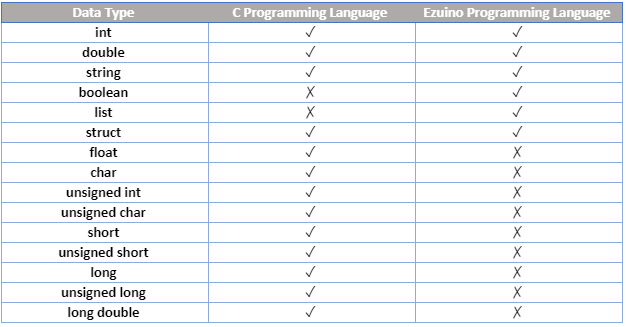
\includegraphics[scale=0.85]{figures/language_features/langf01.png}
\label{lf01}
\end{figure}
\subsubsection*{Bitwise Operators}
In the C programming language, six of its data types, signed and unsigned int char and long, supports for bit manipulation. %The following datatypes are char, int and long (signed and unsigned).
%The different bitwise operators can be found in figure \ref{lf02}:
%\begin{figure}[H]
%\centering
%\caption{Bitwise Operation comparison Arduino C and Ezuino}
%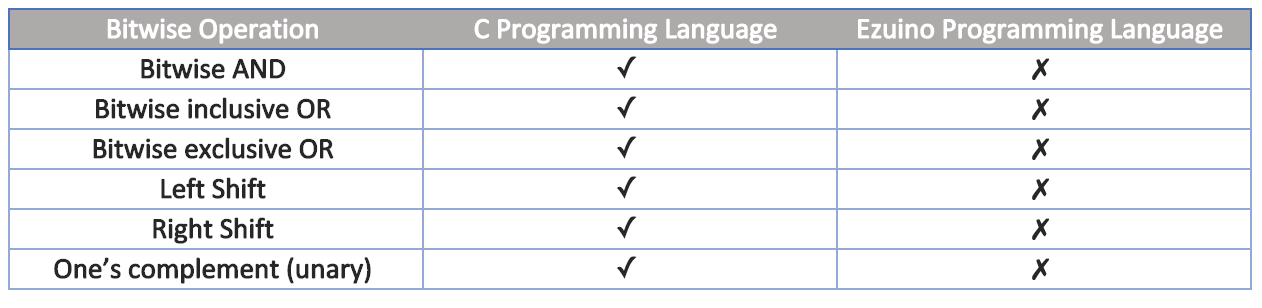
\includegraphics[scale=0.60]{figures/language_features/langf02.png}
%\label{lf02}
%\end{figure}
The reason why the Ezuino Programming language is not using the bitwise operations is that this may require a deeper understanding of how data structures work and require a more in-depth knowledge, which our target group shouldn’t be forced to learn. For our target group this increases readability by increasing the overall simplicity.
\subsubsection*{Logical Operators}
The logical operator is an expression, which is used to express logic in a programming language, and usually returns a boolean expression in the form of true or false. \\
As all three logical operators “AND” “OR” and “!” are an important part to define simple logical expressions, the Ezuino programming language has inherited all the functionality of the C programming language, although we have chosen to change the syntax. To increase writability through expressivity we have chosen to use “and” and “or” instead of \&\& and || that is used in C.\\
\begin{figure}[H]
\centering
\caption{Logical Operation comparison between Arduino C and Ezuino}
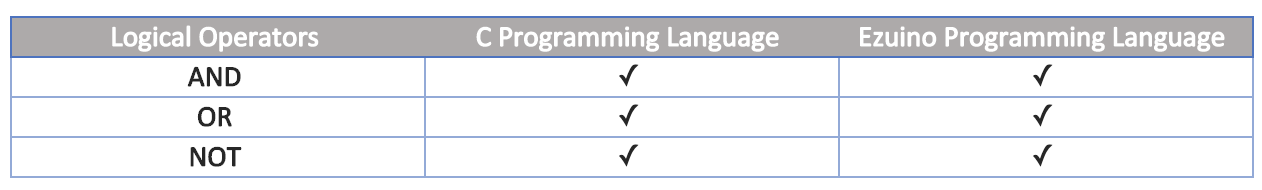
\includegraphics[scale=0.80]{figures/language_features/langf03.png}
\label{lf03}
\end{figure}
\subsubsection*{Relational Operators}
Relational operators define a relationship between two entities, and returns a boolean value.
The Ezuino programming language inherits all the features of C, as with the same case as the Logical Operators, relational operators are an important part of programming language logic. We have chosen to keep the same relational operators as their syntax is very close with the mathematical notations. Compared to C, there will be differences in the equality operator, in Ezuino the syntax will be “=” instead of “==” in C. The different assignment syntax is chosen for its resemblance to mathematical notations in order to increase readability for people unfamiliar with code.
\begin{figure}[H]
\centering
\caption{Relational Operation comparison between Arduino C and Ezuino}
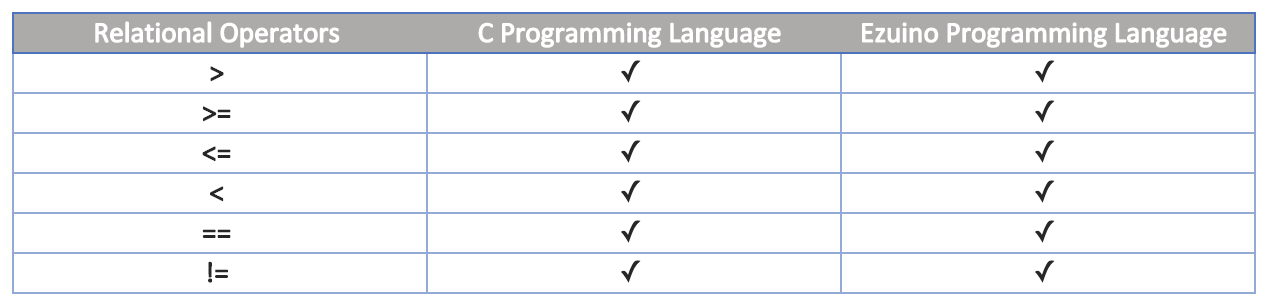
\includegraphics[scale=0.80]{figures/language_features/langf04.png}
\label{lf04}
\end{figure}

\subsubsection*{Arithmetical Operators and Negate}
Arithmetic operators are a necessity for every programming language.
Compared to C we have chosen to not include the modulo operator as it is a fairly programming specific operator not used commonly regular math. Furthermore, the orthogonality in Ezuino makes it possible to define other arithmetic operators as functions if necessary. The modulo operator is easily implemented as a function in our language. Considering these two points, we decided against implementing modulo as an operator.
The "-" sign will also work as negate, converting minus to plus and plus to minus. The functionality of this operator should be fine for people new to programming compared to modulus since it is often used in relatively basic mathematics.
\begin{figure}[H]
\centering
\caption{Arithmetical Operation comparison between Arduino C and Ezuino}
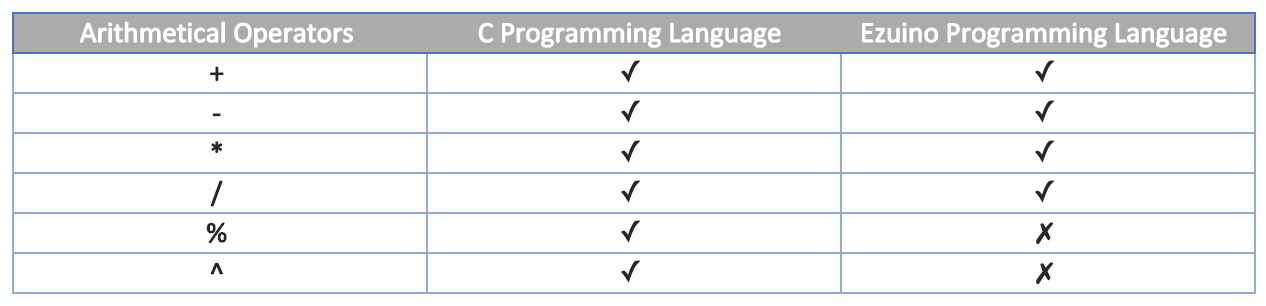
\includegraphics[scale=0.80]{figures/language_features/langf05.png}
\label{lf05}
\end{figure}

\subsubsection*{Pointer Operators}
As described in the problem analysis, most people have difficulty understanding the pointers and address systems, as it requires a sophisticated understanding of how the computer system works. Therefore, it has been decided not to include pointers in the Ezuino programming language. This also prevents most problems in aliasing increasing reliability.
\subsubsection*{Assignment Operators}
A way to assign a value to a variable is essential in any programming language Ezuino has also kept this feature. The syntax will be the one often seen as the mathematical notation for assignment “:=”. Other assignment operators in Arduino C do several operations at once and while these are nice features we regard them as could have features, as they are not essential.
%\begin{figure}[H]
%\centering
%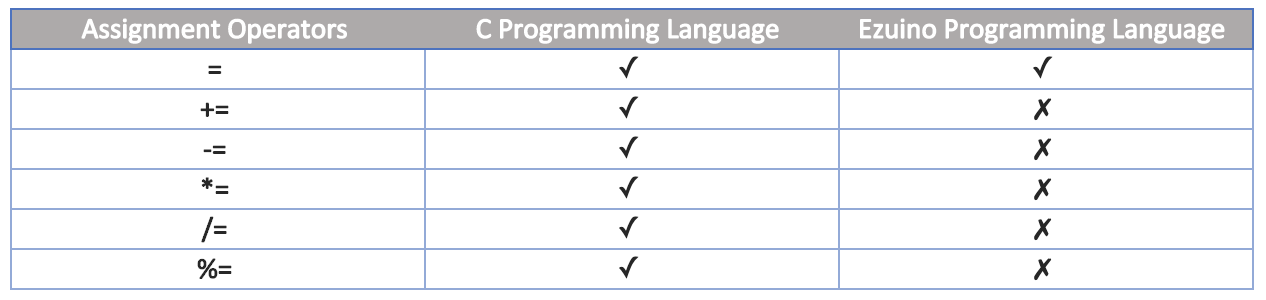
\includegraphics[scale=0.60]{figures/language_features/langf07.png}
%\caption{Assignment Operation comparison between C and Ezuino Programming Language}
%\label{lf07}
%\end{figure}
\subsubsection*{Control Flow}
In the C programming language, control flow statements of a programming language specify the order, in which computations get performed. To add an example, we can use a while loop. The while loop will keep running until a specific condition has not been met. For an example, if an Arduino is set to measure the outside temperature, and the Arduino executes a set of code, while the temperature is below its 20 degrees, the body of the loop will keep running until the temperature rises above 20 degrees. \\
\\
This is the general idea behind control flow. Control flow is a statement which executes of which result is being made as to which of two or more path to follow in a running program. \\
\\
To keep the most essential control flow structures we have chosen to keep the if else commands. We have not chosen to keep else if as it is more niche and if else can cover the same use cases if the use for it is absolutely necessary. This increases overall simplicity at the cost of reduced expressivity.
\\
In regards to loop structures the “while loop” will be the primary loop structure in Ezuono. Although the “for loop” and “do while loop” increase writability people can still do everything they need to in a “while loop”.
%\begin{figure}[H]
%\centering
%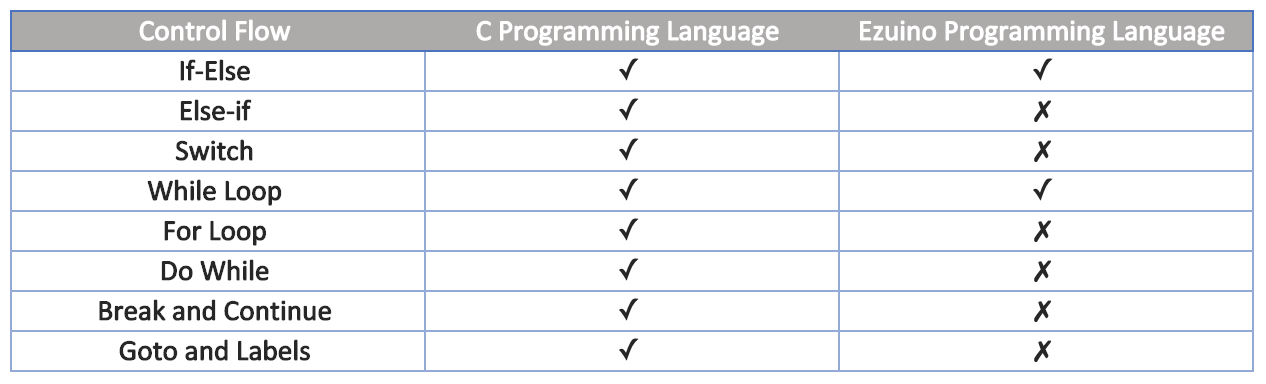
\includegraphics[scale=0.60]{figures/language_features/langf08.png}
%\caption{Control Flow comparison between C and Ezuino Programming %Language}
%\label{lf08}
%\end{figure}
\subsubsection*{Functions and Program Structure}
Functions in the C programming language is commonly used to task large code into smaller, reusable tasks. This enables the users to build and use the function which they have made, instead of writing all the code over again. A right style Arduino C program generally consist of a lot of minor functions, rather than having one significant function.
The basic Arduino functions should also be available in Ezuino, in order to communicate with the Arduino hardware. The ones we plan to implement as a proof of concept are Digital.Read, Digital.Write, Analog.Read, Analog.Write, Pin.Mode, delay, delayMicroseconds, Serial.print Serial.begin and Serial.end. The syntax in Ezuino will be the same albeit without “.” between keywords as we felt that this gave the impression of being object oriented.
\begin{figure}[H]
\centering
\caption{Functions and Program Structure comparison between Arduino C and Ezuino}
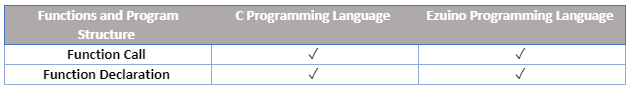
\includegraphics[scale=0.80]{figures/language_features/langf10.png}
\label{lf10}
\end{figure}
When defining the legal program structure there were three options we considered. \\ \\
\subsubsection{Option 1: Using global scope as main}
The global scope could be treated as the main function in Ezuino. This would mean everything inside the global scope should be regarded as legal statements. One of problems with this approach would be that statements and functions could be in arbitrary order. This could easily decrease readability if used improperly.
This would also require that the users would have to implement a while loop to have the same effect as Arduino’s standard loop method, which is often necessary in Arduino programs.
\begin{lstlisting}[caption={Program structure where global scope work as main}, label={lf10}]
int a := 5

func myfunc() {
	a := 8 + 2
}

a := 4
myfunc()
int b := 18
a := b*a

func otherfunc() {
	int c := 321
}

while(true) {
	otherfunc()
}
\end{lstlisting}

\subsubsection{Option 2: Having a main that works as a setup requiring the user to implement his own control structure}
If every statement should be inside main and function declaration should be outside, code would be relatively more orderly and easier to read.
This would however also require that the users implement a while loop if they needed repetition.
\begin{lstlisting}[caption={}, label={}]
func main() {
	int a := 5
	a := 4
	myfunc()
	int b := 10
	a := b*a
	
	while(true) {
		otherfunc()
	}
}

func myfunc() {
	int a := 8 * 2
}

func otherfunc() {
	int c := 321
}
\end{lstlisting}

\subsubsection{Option 3: Using Arduino setup and loop but making loop optional}
Using the same setup method as Arduino is both relatively easy to read as the option 2, but also semantically reminds the user that a repetition is usually needed for Arduino devices by giving it a place that is suitable for grouping such code.
\begin{lstlisting}[caption={Program structure similar to Arduino but where loop is optional}]
func Setup() {
	int a := 5
	a := 4
	myfunc()
	int b := 10
	a := b*a
}

func Loop() {
	otherfunc()
}

func myfunc() {
	int a := 8 * 2
}

func otherfunc() {
	int c := 321
}
\end{lstlisting}

\subsubsection{Chosen program structure for Ezuino}
Because option 2 and 3 both are relatively easier to read than option 1 and because option 3 semantically makes more sense, we chose option 2. Loop should also be optional to follow the design philosophy that extra syntax requirement that decrease writability and are unfriendly to people new to code should not be included.

\subsubsection*{Additional Constructs}
Single line comments will also be possible in Ezuino through \#, as comments are essential for reading code. Print will be available as print have multiple uses and are essential for simple debugging. End of statements will be without ; compared to C in order to increase writability, since it is easier not having to write the extra syntax. Requiring ; also encourages several compound statements on the same line, which reduces readability.
\begin{figure}[H]
\centering
\caption{Additional Constructs comparison Arduino C and Ezuino}
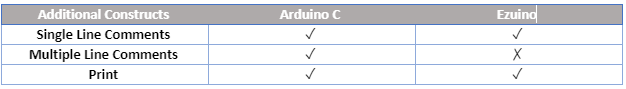
\includegraphics[scale=0.80]{figures/language_features/langf09.png}
\label{lf09}
\end{figure}

\subsection*{Casting}
With the Ezuino language it might be necessary to do casts from one type to another.
The print method should only accept the type string. To make sure that the user really wants to cast, casts have been made explicit.
That means if a user wants to use the print method on an integer, the integer firstly has to be cast to a string in order to print it.
Likewise, casts to the same type cannot be done. The reasoning for this is that it is important to know which types the variables has. If the user isn't aware of the types, it might be difficult to implement the functionality which user wants.\\
%The reason for not including casting from String to other data types is that this requires parsing of the string and as such is not a cast that makes sense.\\
The reason for not including casting from String to other data types is that this would require parsing and this is not the same as casting. One way to do parsing is for example to only accept changing a string to a int is if the string represents a integer. Since parsing strings to other data types have many practical uses but is slightly more time consuming and complex than casting it should be included in Ezuino if there is enough time.  \\
When casting from boolean to integer false will equal 0 and true will equal 1.
In table \ref{tab:cast-overview}, the entire casts can be seen.
\begin{table}[H]
\centering
\begin{tabular}{lllll}
To\textbackslash From & String   & Integer      & Double       & Boolean      \\
String                & $\times$ & $\checkmark$ & $\checkmark$ & $\checkmark$ \\
Integer               & $\times$ & $\times$     & $\checkmark$ & $\checkmark$ \\
Double                & $\times$ & $\checkmark$ & $\times$     & $\checkmark$ \\
Boolean               & $\times$ & $\checkmark$ & $\times$     & $\times$    
\end{tabular}
\caption{List over casts in Ezuino. Casts marked with $\checkmark$ are valid, $\times$ marks invalid casts}
\label{tab:cast-overview}
\end{table}